%%%%%%%%%%%%%%%%%%%%%%%%%%%%%%%%%%%%%%%%
% Classe do documento
%%%%%%%%%%%%%%%%%%%%%%%%%%%%%%%%%%%%%%%%

% Nós usamos a classe "unb-cic".  Deixe apenas uma das linhas
% abaixo não-comentada, dependendo se você for do bacharelado ou
% da licenciatura.

\documentclass[bacharelado]{unb-cic}
%\documentclass[licenciatura]{unb-cic}



%%%%%%%%%%%%%%%%%%%%%%%%%%%%%%%%%%%%%%%%
% Pacotes importados
%%%%%%%%%%%%%%%%%%%%%%%%%%%%%%%%%%%%%%%%

\usepackage[brazil,american]{babel}
\usepackage[T1]{fontenc}
\usepackage{indentfirst}
\usepackage{natbib}
\usepackage{xcolor,graphicx,url}
\usepackage[utf8]{inputenc}
\usepackage{bm}
\usepackage{listings}
\usepackage{csquotes}



%%%%%%%%%%%%%%%%%%%%%%%%%%%%%%%%%%%%%%%%
% Cores dos links
%%%%%%%%%%%%%%%%%%%%%%%%%%%%%%%%%%%%%%%%

% Veja o arquivos cores.tex se quiser ver que outras cores estão
% pré-definidas.  Utilizando o comando \hypersetup abaixo nós
% evitamos aquelas caixas vermelhas feias em volta dos links.

%%%%%%%%%%%%%%%%%%%%%%%%%%%%%%%%%%%%%%%%
% Cores do estilo Tango
%%%%%%%%%%%%%%%%%%%%%%%%%%%%%%%%%%%%%%%%

\definecolor{LightButter}{rgb}{0.98,0.91,0.31}
\definecolor{LightOrange}{rgb}{0.98,0.68,0.24}
\definecolor{LightChocolate}{rgb}{0.91,0.72,0.43}
\definecolor{LightChameleon}{rgb}{0.54,0.88,0.20}
\definecolor{LightSkyBlue}{rgb}{0.45,0.62,0.81}
\definecolor{LightPlum}{rgb}{0.68,0.50,0.66}
\definecolor{LightScarletRed}{rgb}{0.93,0.16,0.16}
\definecolor{Butter}{rgb}{0.93,0.86,0.25}
\definecolor{Orange}{rgb}{0.96,0.47,0.00}
\definecolor{Chocolate}{rgb}{0.75,0.49,0.07}
\definecolor{Chameleon}{rgb}{0.45,0.82,0.09}
\definecolor{SkyBlue}{rgb}{0.20,0.39,0.64}
\definecolor{Plum}{rgb}{0.46,0.31,0.48}
\definecolor{ScarletRed}{rgb}{0.80,0.00,0.00}
\definecolor{DarkButter}{rgb}{0.77,0.62,0.00}
\definecolor{DarkOrange}{rgb}{0.80,0.36,0.00}
\definecolor{DarkChocolate}{rgb}{0.56,0.35,0.01}
\definecolor{DarkChameleon}{rgb}{0.30,0.60,0.02}
\definecolor{DarkSkyBlue}{rgb}{0.12,0.29,0.53}
\definecolor{DarkPlum}{rgb}{0.36,0.21,0.40}
\definecolor{DarkScarletRed}{rgb}{0.64,0.00,0.00}
\definecolor{Aluminium1}{rgb}{0.93,0.93,0.92}
\definecolor{Aluminium2}{rgb}{0.82,0.84,0.81}
\definecolor{Aluminium3}{rgb}{0.73,0.74,0.71}
\definecolor{Aluminium4}{rgb}{0.53,0.54,0.52}
\definecolor{Aluminium5}{rgb}{0.33,0.34,0.32}
\definecolor{Aluminium6}{rgb}{0.18,0.20,0.21}

\hypersetup{
  colorlinks=true,
  linkcolor=DarkScarletRed,
  citecolor=DarkScarletRed,
  filecolor=DarkScarletRed,
  urlcolor= DarkScarletRed
}



%%%%%%%%%%%%%%%%%%%%%%%%%%%%%%%%%%%%%%%%
% Informações sobre a monografia
%%%%%%%%%%%%%%%%%%%%%%%%%%%%%%%%%%%%%%%%

\title{Armazenamento de Dados Abertos com NoSQL}

\orientador{\prof[a] \dr[a] Maristela Terto de Holanda}{CIC/UnB}
%\coorientador[a]{\prof[a] \dr[a] Coorientadora}{MAT/UnB}
\coordenador{\prof \dr Flávio de Barros Vidal}{CIC/UnB}
\diamesano{15}{dezembro}{2016}

\membrobanca{\prof \dr Professor I}{CIC/UnB}
\membrobanca{\prof \dr Professor II}{CIC/UnB}

\autor{Jorge Luiz}{Andrade}
\CDU{004.4}

\palavraschave{bancos de dados, nosql, dados abertos }
\keywords{databases, nosql, open data}



%%%%%%%%%%%%%%%%%%%%%%%%%%%%%%%%%%%%%%%%
% Texto
%%%%%%%%%%%%%%%%%%%%%%%%%%%%%%%%%%%%%%%%

\begin{document}
  \maketitle
  \pretextual

  \begin{dedicatoria}
  Dedico a....
  \end{dedicatoria}

  \begin{agradecimentos}
  Agradeço a....
  \end{agradecimentos}

  \begin{resumo}
  A ciência...
  \end{resumo}

  \selectlanguage{american}
  \begin{abstract}
  The science...
  \end{abstract}
  %\selectlanguage{brazil}

  \tableofcontents
  \listoffigures
  \listoftables

  \textual
  \chapter{Introdução}

Dados abertos tem ganhado importância cada vez maior em nossa sociedade. O volume desses dados, que podem ser definidos como dados livres para acesso, utilização e modificação~\cite{opendefinition}, tem crescido cada vez mais, e vem sendo necessário encontrar novas formas para realizar o seu armazenamento e analise, comumente realizados por meio de bancos de dados.

Bancos de dados podem ser definidos como um conjunto de dados que se relazionam entre si e armazenados de forma que possam ser acessados posteriormente, quando necessario~\cite{leavitt2010nosql}.
Os bancos de dados relacionais predominaram por pelo menos nas últimas três décadas, mas seu desempenho em certas aplicações atuais, principalmente naquelas que trabalham com grande volumes de dados, denominado \emph{Big Data}, vem sendo questionado. 

Esse questionamento levou à criação do movimento NoSQL, um novo paradigma de armazenamento de dados que ignora certas restrições dos bancos relacionais tradicionais e tentam melhorar seu armazenamento e desempenho por meio de um sistema distribuído em \emph{clusters}.

A utilização de bancos NoSQL para o tratamento de grande volumes de dados provenientes de dados abertos é uma possibilidade a ser analisada, a fim de permitir um acesso mais fácil e rápido por parte da população. 









  \chapter{Introdução}

Podemos definir um banco de dados relacional como um conjunto de dados que se relacionam entre si, armazenados de uma forma persistente, ou seja, que possam ser recuperados quando necessários. Devido às suas características de persistência, concorrência, integração e padronização, tem sido o modelo padrão de armazenamento, principalmente em ambientes empresariais, a pelo menos vinte anos na computação\cite{pramod}. Uma questão importante em bancos de dados computacionais atuais é a não necessidade que o usuário tem de conhecer como esses dados são armazenados. Isso é possível graças aos chamados Sistemas Gerenciadores de Bancos de Dados(SGBDs)\cite{jan}.

\section{NoSQL}
Nos últimos anos, devido a novas necessidades, tem surgido um movimento em direção a um novo paradigma denominado NoSQL. O termo foi utilizado pela primeira vez em 1998 para denominar um banco de dados que omitia o uso de SQL. A definição atual, porém, tem suas bases em uma reunião realizada em 2009 em São Franscisco, Estados Unidos. Organizada por Johan Oskarsdon, criador do Last.fm, nela foram discutidas formas mais eficientes e baratas de organização dos dados, como as já sugeridas pelo Google Bigtable e Amazon's Dynamo em publicações anteriores\cite{chrisnosql}.

O termo não tem uma definição precisa e universalmente aceita, mas é geral descrito como "Not Only SQL". Bancos NoSQL em geral são caracterizados, mas não definidos, como sendo não relacionais, sem esquema bem definido e distribuidos, favorecendo a execução em clusters, apesar de existirem excessões, como os bancos de dados de grafos, que são executados geralmente em um único servidor.

Bancos de dados NoSQL possuem padrões de modelos de dados, que compartilham certas características em comum e servem a determinadas aplicações específicas, podendo alguns bancos serem classificados em mais de uma categoria. A tabela \ref{tab:modelosnosql} lista os quatro modelos atuais e alguns bancos de dados que se enquadram em cada um deles.

~\begin{table}[]
\centering
\caption{Modelos de Bancos NoSQL}
\label{tab:modelosnosql}
\begin{tabular}{ll}
\textbf{Modelo de Dados}     & \textbf{Exemplo de bancos de dados}      \\ \hline
Chave-valor         & Project Voldemort               \\
                    & Riak                            \\
                    & BerkeleyDB                      \\ \hline
Documentos          & CouchDB                         \\
                    & MongoDB                         \\
                    & OrientDB                        \\ \hline
Famílias de colunas & Cassandra                       \\
                    & HBase                           \\ \hline
Grafos              & Neo4j, OrientDB, Infinite Graph \\
                    & OrientDB                        \\
                    & Infinite Graph                 
\end{tabular}
\end{table}

\section{Dados Abertos}
A Open Definition define um dado como aberto "se qualquer pessoa esta livre para acessá-lo, utilizá-lo, modificá-lo, e compartilhá-lo — restrito, no máximo, a medidas que preservam a proveniência e abertura."\cite{opendefinition}.

O poder público brasileiro vem nos últimos anos realizando ações que promovem a abertura de dados governamenais. Essas ações visam benefícios como melhoria da gestão pública, transparência, controle a participação social, geração de emprego e renda e estímulo à inovação tecnológica. \cite{tcu}. Para atingir esse fim, no ano de 2012 foi definido, em instrução normativa, a implantação da INDA, Infraestrutura Nacional de Dados Abertos, "um conjunto de padrões, tecnologias, procedimentos e mecanismos de controle necessários para atender às condições de disseminação e compartilhamento de dados e informações públicas no modelo de Dados Abertos"\cite{inda}.  












  \chapter{Diferenças entre Bancos de Dados Relacionais e NoSQL}

O armazenamento a a manipulação de dados tem sido um importante foco da computação desde o seu nascimento, tendo os bancos de dados suas raízes já na década de 60, principalmente em aplicações médicas e científicas~\cite{neufeld1986database}, e em 1970, Edgar Codd propos uma nova forma de armazenamento de dados, que ficou conhecida como modelo de dados relacionais (\emph{relational model of data})~\cite{codd1970relational}. 

\section{Bancos de Dados Relacionais}
    Podemos definir um banco de dados relacional como um conjunto de dados que se relacionam entre si e que são armazenados de forma persistente, podendo ser recuperados quando necessário. Os dados são armazenados em tabelas, que são organizadas por colunas, que definem uma categoria de um dado, e por linhas, que representam a instância de um dado~\cite{leavitt2010nosql}. A popularização desse modelo em virtude de suas características de persistência, concorrência e integração entre múltiplas aplicações, o transformou no modelo padrão de armazenamento computacional, principalmente em ambientes empresarias~\cite{pramod}. Outra questão de importância em bancos de dados computacionais é a não necessidade que o usuário tem de conhecer como esses dados são armazenados, o que foi possível com o uso dos chamados Sistemas Gerenciadores de Bancos de Dados (SGBDs)~\cite{jan}.
    
    Outras opções surgiram ao longo dos anos, como os bancos orientados a objetos ou bancos XML. Nenhum deles, entretanto, conseguiu competir com o modelo ja tradicional de dados relacionais.~\cite{pramod} Nos últimos anos, entretanto, o modelo conhecido como NoSQL vem surgindo como essa alternativa.

\subsection{Propriedades ACID}
	Interações com bancos de dados relacionais tradicionais são feitas por meio de transações, que podem ser definidas como operações de leitura e escrita que devem ocorrer de forma independente umas das outras~\cite{dmsbook}. Para garantir que isso ocorra, um SGBD deve prover as seguintes propriedades, conhecidas como propriedades ACID~\cite{haerder}:
	\begin{itemize}
	\item \textbf{Atomicidade}, onde uma determinada transação deve ser feita em sua totalidade, ou seja, todas as operações de que dela fazem parte devem ser bem sucedidas.
	\item \textbf{Consistência} diz que após cada transação, o estado do banco permanece consistente ao seu modelo.
	\item \textbf{Isolamento} garante que cada transação é executada independentemente de outras que estejam ocorrendo em concorrência.
	\item \textbf{Durabilidade} que define que o resultado de uma transação bem sucedida é persistido no banco, mesmo na eventualidade de falhas no sistema.
	\end{itemize}

	Essas propriedades, ao mesmo tempo que garantem a validade do esquema e dos dados em um banco, sacrificam desempenho e disponibilidade, características importantes em várias aplicações atuais~\cite{foxcluster}.

\section{Bancos NoSQL}
    O rápido crescimento no volume de dados nos últimos anos, principalmente após a bolha da Internet na década de 90~\cite{pramod}, trás uma necessidade de certa mudança em relação ao modelo tradicional.
    
    Apesar das vantagens já citada, esse modelo tem restrições principalmente em questões de escalabilidade, complexidade dos dados e rigidez em seus esquemas~\cite{leavitt2010nosql}. Isso levou ao surgimento de um movimento em direção ao novo paradigma denominado NoSQL. O termo foi utilizado pela primeira vez em 1998 para denominar um banco de dados que omitia o uso de SQL. A definição atual, porém, tem suas bases em uma reunião realizada em 2009 em São Franscisco, Estados Unidos. Organizada por Johan Oskarsdon, criador do Last.fm, nela foram discutidas formas mais eficientes e baratas de organização dos dados, como as já sugeridas em publicações anteriores, como o Google Bigtable em 2006~\cite{bigtable}, e Amazon's Dynamo em 2007~\cite{dynamo, chrisnosql}.
\subsection{Definição e Características}
Apesar do termo não tem uma definição precisa e universalmente aceita, sendo geralmente descrito como \emph{Not Only SQL}, bancos NoSQL em geral são caracterizados, mas não definidos, como sendo não relacionais, sem esquema bem definido e distribuidos~\cite{pramod}.
	Entre as razões e vantagens dos bancos NoSQL podemos citar~\cite{chrisnosql}:
    \begin{itemize}
    \item \textbf{Evitar complexidade desnecessária}: Bancos relacionais costumam aderir às já citadas propriedades ACID, além de serem restritos em seu esquema de dados. Bancos NoSQL costumam ignorar ou relaxar essas restrições a fim de obter um melhor desempenho.
    \item \textbf{Alto rendimento}: Bancos NoSQL surgiram da necessidade e armazenamento e processamento de um cada vez maior volume de dados, e por isso são construídos objetivando um desempenho melhor, em aplicações específicas, do que de bancos tradicionais.
    \item \textbf{Alta escalabilidade}: Bancos relacionais podem ser escalados verticamente com a utilização de equipamentos poderosos e caros, e uma operação distribuida costuma ser mais complexa devido à forma de armazenamento de seus dados~\cite{leavitt2010nosql}. Bancos NoSQL foram pensados para execução em um sistema de \emph{clusters}, o que facilita a sua escalabilidade horizontal e reduz a necessidade de um hardware mais caro e específico, podendo ser utilizado em \emph{hardwares} mais simples. 
    \item \textbf{Alta disponibilidade}: Devido à possibilidade de escalabilidade horizontal, bancos NoSQL podem distribuir sua operação em diversos nós de um \emph{cluster}, o que possibilita acesso simultâneo por um grande número de usuários, mesmo que não seja possível acessar algum desses nós. 
    \item \textbf{\emph{Open source}}: SGBDs tradicionais costumam possuir licenças pagas, gerando um custo financeiro alto, principalmente quando executados em múltiplas máquinas~\cite{pramod}. NoSQLs costumam seguir licenças \emph{open source}, podendo reduzir significativamente os gastos da aplicação. 
\end{itemize}

\subsection{Teorema CAP}
	Em 2000, foi proposto o teorema CAP, que define limitações em sistemas distribuidos. O teorema define que podemos garantir somente duas das seguintes três propriedades em um determinado sistema: Consistência (\emph{Consistency}) , Disponibilidade (\emph{Availability}) e Tolerância a partições (\emph{Partition-resilience})~\cite{brewer}. Essas propriedades podem ser definidas como:
    \begin{itemize}
	\item \textbf{Consistência} define que todos os nós possuem os mesmos dados em qualquer dado instante, e um pedido de leitura em qualquer desses nodos garante o dado mais atual possível do sistema.
    \item \textbf{Disponibilidade} garante é sempre possível ler e gravar dados em um nodo dado que ele está acessível. 
    \item \textbf{Tolerância a partições} garante que o sistema irá continuar funcionando mesmo na hipótese de eventuais falhas de comunicação entre os nodos.
	\end{itemize}
	
    Essas propriedades podem ser agrupadas da seguinte forma e obtendo os seguintes resultados:
    \begin{itemize}
    \item \textbf{CA sem P} são sistemas distribuídos cujos nós estejam em uma mesma partição de rede.
    \item \textbf{CP sem A} são sistemas que, em caso de falha em pelo menos um dos nós, ficam indisponíveis até sua total recuperação. Bancos de Dados que seguem as propriedades ACID costumam seguir esse padrão.
    \item \textbf{AP sem C} são sistemas que devem permanecer em funcionamento mesmo durante uma eventual falha em um ou mais de seus nós, mesmo que isso resulte em dados não atualizados durante consultas. Sistemas NoSQL costumam seguir esse padrão.  
	\end{itemize}
    
    Sistemas distribuídos em grandes áreas, por estarem sempre sujeitos a falhas de rede~\cite{deutsch}, não podem ignorar a Tolerância a Falhas, tendo de fazer uma escolha entre Consistência e Disponibilidade~\cite{brewer12years}.
    
    A figura \ref{fig:capnosql} ilustra as diferentes combinações das propriedades CAP e exemplos de bancos de dados que as utilizam.
    

\begin{figure}[!htb]
\centering
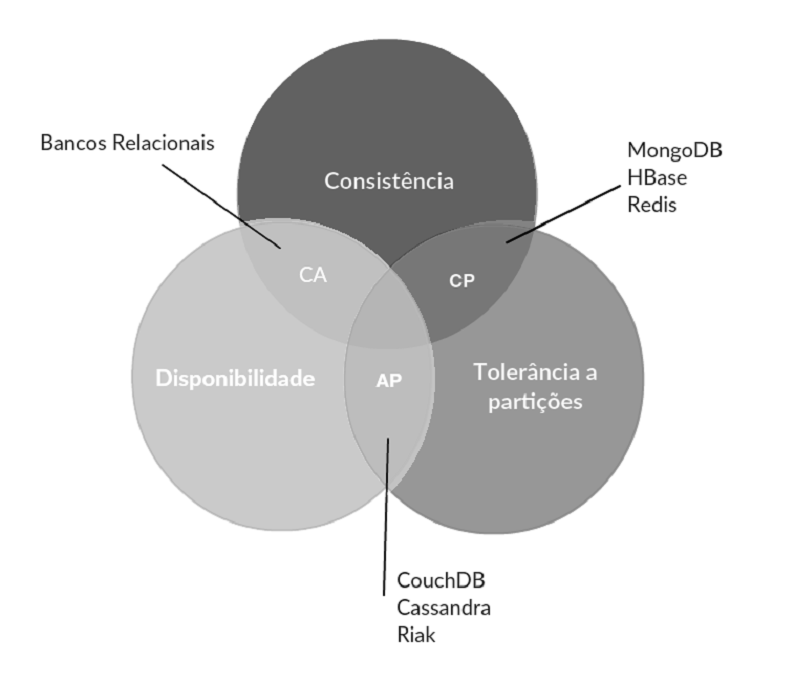
\includegraphics[width=0.65\textwidth]{figuras/cappb.png}
\caption{Propriedades CAP e exemplos. Adaptado de ~\cite{blograshid}}
\label{fig:capnosql}
\end{figure}

\subsection{BASE}
    Em um ambiente distribuido, escabalibilidade, resiliência e velocidade são mais importantes do que consistência imediata e segurança quanto à veracidade dos  dados, não sendo necessária a aderência total às propriedades ACID já citadas~\cite{neo4j_acidbase}. Além disso, de acordo com o \textbf{Teorema CAP}, um banco que aceite particionamento não pode possuir alta disponibilidade e consistência simultâneamente. Essa necessidade, tanto de performance quanto de disponibilidade, levou à criação do acrônimo \textbf{BASE}, \emph{\textbf{B}asically \textbf{A}vailable} (Basicamente Disponível), \emph{\textbf{S}oft State} (Estado Leve) e \emph{\textbf{E}ventual Consistency} (Consistência Eventual)~\cite{foxcluster}. 
    
    Enquanto um banco \textbf{ACID} é pessimista, requerendo que cada operação mantenha a consistência do banco como um todo, \textbf{BASE} segue uma visão otimista, entendendo que dados serão eventualmente consistentes.
    
    Sistemas distribuídos costumam manter cópias de dados em várias máquinas em um \emph{cluster} para aumentar a sua disponibilidade, e quando um desses dados é atualizado em uma dessas máquinas é natural que haja um intervalo de tempo até que todas essas cópias sejam atualizadas.

\subsection{Modelos NoSQL}
Bancos de dados NoSQL possuem padrões de modelos de dados, que compartilham certas características em comum e servem a determinadas aplicações específicas, podendo alguns bancos serem classificados em mais de uma categoria. A tabela \ref{tab:modelosnosql} lista os quatro modelos atuais e alguns bancos de dados que se enquadram em cada um deles.

~\begin{table}[]
\centering
\caption{Modelos de Bancos NoSQL}
\label{tab:modelosnosql}
\begin{tabular}{ll}
\textbf{Modelo de Dados}     & \textbf{Exemplo de bancos de dados}      \\ \hline
Chave-Valor         & Project Voldemort               \\
                    & Riak                            \\
                    & Redis                           \\
                    & BerkeleyDB                      \\ \hline
Documentos          & CouchDB                         \\
                    & MongoDB                         \\
                    & OrientDB                        \\ \hline
Famílias de colunas & Cassandra                       \\
					& Hypertable                      \\
                    & HBase                           \\ \hline
Grafos              & Neo4j \\
                    & OrientDB                        \\
                    & Infinite Graph                 
\end{tabular}
\end{table}

\subsection*{Chave-Valor}
Bancos com armazenamento em chave-valor existem a muito tempo, como \emph{Berkeley DB}, mas ganharam importância no meio NoSQL a partir do Amazon DynamoDB e do Google BigTable~\cite{chrisnosql}.

Consiste basicamente em uma tabela \emph{hash}, sendo o acesso aos dados realizado por meio de uma chave primária, assim como ocorre em \emph{maps} e dicionários.  Esses bancos são completamente livres de esquema e suas operações se resumem a consultar o valor a partir de uma chave, inserir um valor para uma chave ou deletar uma chave e seu valor do banco~\cite{nosqleval}. O valor armazenado em geral pode representar qualquer tipo de objeto, como uma \emph{string} ou um \emph{BLOB}, não sendo necessária que exista qualquer relação entre diferentes registros, ficando a aplicação responsável pelo seu tratamento. 

Esses bancos favorecem escalabilidade sobre consistência, e por isso em geral não possuem ferramentas mais poderosas de consulta e análise de dados~\cite{chrisnosql}.

Atualmente temos como exemplos de bancos chave-valor: \emph{Riak}, \emph{Redis}, \emph{Berkeley DB} e \emph{Project Voldemort}.

\subsection*{Documentos}
Bancos orientados a documentos armazenam seus dados em forma de documentos, podendo esses terem formato \emph{XML}, \emph{JSON}, \emph{BSON}, etc~\cite{pramod}. Podem ser vistos como a sequência natural do armazenamento por chave-valor, ainda fazendo o armazenamento por meio de um par chave-valor, mas utilizando uma estrutura mais rica para armazenamento dos dados ao armazenar um documento na parte do valor~\cite{chrisnosql}. Cada um desses documentos pode ter certa semelhança uns com os outros, mas não necessitam possuir a mesma estrutura, o que permite uma grande flexibilidade no esquema do banco.

A seguir temos um exemplo de dois documentos. Apesar de parecidos, eles possuem certas diferenças, o que gera essa grande flexibilidade do modelo orientado a documentos.

\begin{lstlisting}
{
  "clienteid" : "f6a6fs86fa",
  "cliente" :
  {
    "primeironome" : "Pedro",
    "sobrenome" : "Silva", 
    "gosta" : ["Leitura", "Viagem"]
  }
  "endereco" : 
  {
    "estado" : "Sao Paulo",
    "cidade" : "Guarulhos"
  }
}

{
  "clienteid" : "ga9s8g8fe",
  "cliente" :
  {
    "primeironome" : "Maria",
    "sobrenome" : "Costa", 
    "gosta" : ["Esportes"]
  }
  "ultimaCompra" : "12/11/2015"
}
\end{lstlisting}

Esses documentos não são opacos à aplicação, seu conteúdo pode ser consultado diretamente, com consultas diretas em atributos de seus registros. Isso permite a manipulação de estruturas mais complexas, que ainda assim não possuem nenhuma restrição de esquema, sendo fácil a inserção de novos documentos ou a modificação dos documentos já armazenados. Devido à essa flexibilidade, são recomendados para integração de dados e migração de esquemas~\cite{nosqleval}. 

Como exemplos de bancos orientados a documentos podemos citar o \emph{CouchDB}, \emph{MongoDB} e \emph{OrientDB}.

\subsection*{Colunas}
Bancos de Dados colunares tem sua influência no \emph{Google BigTable}~\cite{bigtable}, e armazenam seus dados em famílias de colunas que são associadas a uma chave de linha. Cada uma dessas famílias de colunas pode possuir várias colunas, e são consideradas dados relacionados que podem ser acessados ao mesmo tempo~\cite{pramod}. 

O Cassandra possui ainda o conceito de super colunas, que pode ser visto como um agrupamento de colunas que pode ser armazenado dentro de uma família de colunas~\cite{pramod}.

Colunas e linhas podem ser adicionadas a qualquer momento, o que gera uma flexibilidade bem maior em relação aos esquemas em geral fixos dos bancos de dados relacionais.  Entretanto, famílias de colunas em geral devem ser predefinidas, situação menos flexível que a encontrada nos modelos de chave-valor ou de documentos~\cite{nosqleval}.  

Como exemplo de bancos orientados a colunas temos o \emph{HBase} e \emph{Hypertable}, que são implementações \emph{open source} do BigTable, e o \emph{Cassandra}.


\subsection*{Grafos}
Diferente dos bancos relacionais e dos já citados modelos NoSQL vistos, um banco de dados em grafos é especializado em dados altamente conectados. São ideias para aplicações que realizam consultas baseadas em relações~\cite{nosqleval}.
Esse modelo realiza o armazenamento por meio de entidades e os relacionamentos entre essas entidades. Entidades podem ser vistas como nós e os relacionamentos como as areas de um grafo~\cite{pramod}. Esses nós podem possuir propriedades dos objetos que representam, assim como as áreas, que podem possuir atributos do relacionamento e além disso possuem significância em sua direção.

Consultas nesse tipo de modelo são realizadas percorrendo o grafo. Isso possui como vantagem a possibilidade de se modificar a forma que se camanha nesse grafo, sem ser necessárias mudanças em sua estrutura de nós e relações~\cite{pramod}.

Uma diferença importante dos bancos orientados a grafos em relação aos modelos anteriores é o seu suporte menor a sistemas distribuidos, não sendo geralmente possível a distribuição dos nós em diferentes servidores~\cite{pramod}.

Como exemplos desse modelo podemos citar o \emph{Neo4J}, o \emph{Infinite Graph} e o \emph{OrientDB}.
  \chapter{Cassandra}

Esse trabalho ira utilizar o Cassandra como banco de dados para validação de sua hipótese. Como visto no capítulo 3, o Apache Cassandra, distribuição que sera utilizada, é um banco de dados orientado a colunas altamente disponível e distribuído em servidores constituídos de hardware de \enquote{prateleira} para gerenciamento de grande volumes de dados~\cite{lakshmancassandra}. Este capítulo tem como objetivo definir esse banco de dados, suas características, funcionamento, vantagens e desvantagens.

\section{Definição}
O Cassandra se originou em 2007 como um projeto do \emph{Facebook} para resolver um problema na busca da caixa de mensagens. A compania necessitava de um sistema com alta performance, confiabilidade, eficiência e que suportasse o contínuo crescimento da ferramenta~\cite{lakshmancassandra, cassandraguide}. 

O projeto foi desenvolvido por Jeff Hammerbacher, Avinash Lakshman, Karthik Ranganathan e Prashant Malik, tendo seu modelo de dados sofrido grande inspiração nos trabalhos anteriores do \emph{Amazon Dynamo}~\cite{dynamo} e do \emph{Google Bigtable}~\cite{bigtable}, e lançado em 2008 como um projeto \emph{open source}. Foi mantido e atualizado apenas pelo Facebook até 2009, quando foi comprado pela Apache~\cite{cassandraguide}, sendo utilizado atualmente por companias como \emph{Netflix}, \emph{Spotify} e até em agências governamentais, como a NASA~\cite{cassandracompanies}. 

Pode ser definido como um banco de dados orientado a colunas \emph{open source}, distribuído, descentralizado, elasticamente escalavel, altamente disponível, tolerante a falhas e variavelmente consistente~\cite{cassandraguide}. A seguir iremos analisar cada uma dessas características.

\subsection{Características}

\subsection*{Distribuído e Descentralizado}
O Cassandra é capaz de ser executado em múltiplas de forma transparente ao usuário, que o enxerga como um sistema unificado. Apesar de ser possível sua execução em um único nó, só é possível obter algum benefício com uma execução distribuída. Além do ganho de performance, a distributividade do sistema garante maior segurança devido à redundância de dados.

Diferente de outros bancos distribuidos que elegem nós como mestres e escravos, o Cassandra opera de forma descentralizada, o que significa que todos os nós são idênticos em sua forma de execução, sendo utilizados protocolos \emph{peer-to-peer} (par-a-par) e \emph{gossip} para manutenção e sincronia entre os nós. Essa descentralização garante que não exista apenas um ponto de falha, o que aumenta sua disponibilidade, e simplifica a operação do e manutenção do \emph{cluster}.

\subsection*{Elasticamente Escalável}
Escalabilidade é a propriedade que um sistema tem de atender um crescente número de requisições sem prejuízo de performance. Essa escalabilidade pode ser tanto vertical quanto horizontal. Na escalabilidade vertical o hardware já utilizado no sistema é melhorado, enquanto na escalabilidade horizontal novos máquinas são adicionadas à arquitetura, havendo a divisão da carga do sistema.

O Cassandra possui escalabilidade horizontal elástica, o que significa que sua arquitetura pode escalar tanto para cima quanto para baixo. Na necessidade de uma melhora do desempenho da aplicação, novas máquinas podem ser adicionadas, e o Cassandra se encarrega de fazer a distribuição dos dados de forma transparente, sem necessidade de configurações adicionais ou reiniciamento do sistema. Da mesma forma, em caso de necessidade, máquinas podem ser retiradas do \emph{cluster} sem prejuizo ao todo, devido ao rebalanceamento automático.

\subsection*{Altamente disponível e Tolerante a falhas}
A disponibilidade de um sistema é medida de acordo com sua capacidade de responder a requisições. Computadores, e especialmente sistemas distribuídos em rede, estão sujeitos a falhas, que em geral só podem ser contornadas por meio de sistemas redundantes.

Devido a replicação e redundância de dados e a sua capacidade de substituição de nós indisponíveis, o Cassandra pode ser definido como um sistema altamente disponível e tolerante à falhas em suas máquinas.

\subsection*{Variavelmente Consistente}
A consistência de uma aplicação diz respeito à sua capacidade de retornar o valor mais atual em uma requisição.

Como visto no Teorema CAP\ref{sec:cap}, não é possível a um sistema ser totalmente conscistente, disponível e tolerante a falhas. 

O Cassandra é por vezes definido como \enquote{eventualmente consistente}, por trocar parte de sua consistência por alta disponibilidade. Essa definição, porém, não é totalmente correta, e um termo melhor para defini-lo é \enquote{variavelmente consistente} (\emph{tuneably consistent}), podendo essa sua consistência ser ajustada de acordo com o tipo de aplicação.

\section{Modelo de Dados}

Um banco de dados Cassandra consiste em um \emph{keyspace}, formado por colunas agrupadas em conjuntos chamados famílias de colunas. Esse modelo é bastante semelhante ao que foi proposto pelo Bigtable~\cite{lakshmancassandra, bigtable}. Seu modelo de dados pode ser visto como um mapa multidimensional indexado por uma chave, se assemelhando aos modelos de chave-valor e orientados à colunas. A seguir veremos em detalhes cada um desses conceitos.

\subsection*{\emph{Keyspace}}
Um \emph{keyspace} define o maior agrupamento de dados no Cassandra, podendo ser correspondido a um banco de um SGBD relacional. Um \emph{keyspace} define um nome e uma série de atributos que definem o seu comportamento~\cite{cassandraguide}.

Atributos do \emph{keyspace} incluem:
\begin{itemize}
\item \textbf{Fator de replicação} diz respeito ao número de nós que armazenarão uma réplica de cada linha de dados. O fator de replicação tem forte influencia no balanço entre performance e consistência do banco de dados.
\item \textbf{Estratégia de replicação} se refere a como as réplicas (ou cópias) de um dado serão posicionados no anel do \emph{cluster}.
\item \textbf{Famílias de colunas} pode ser visto como o análogo às tabelas de um modelo relacional, da mesma forma que o \emph{keyspace} é o análogo do banco.  Uma família de colunas é um agrupamento para uma coleção de linhas, onde cada linha contém colunas ordenadas.
\end{itemize}

\subsection*{Colunas e famílias de colunas}
Uma família de colunas (ou tabela) no Cassandra é um mapa multidimensional indexado por uma chave. Essa chave é uma \emph{string} sem restrição de tamanho, mas que em geral varia de 16 a 36 \emph{bytes}. O valor desse mapeamento consiste em uma família de colunas, um agrupamento para uma coleção ordenadas de linhas, que por sua vez é uma coleção ordenada de colunas ~\cite{lakshmancassandra, cassandraguide}.

O modelo de família de colunas se diferencia do modelo relacional por ser o que é chamado comumente de \emph{livre de esquema} (\emph{schama free}) . É possível realizar a inserção, remoção ou alteração de qualquer coluna ou família de colunas a qualquer momento, ficando as aplicações clientes do banco encarregadas de interpretar e manipular o novo modelo de dados. 

Ao se inserir um novo dado em uma família de colunas do Cassandra são especificados valores para uma ou mais colunas. O conjunto de valores é chamado de linha, e é identificado unicamente por uma chave de linha. Uma linha não precisa possuir dados para todas colunas presentes na família de colunas à que ela pertence, sendo o espaço alocado apenas para as colunas presentes nessa linha. Isso gera tanto uma economia de espaço quanto uma melhora de performance em relação a um banco relacional, que precisa preencher com valores nulos colunas não utilizadas.

  % \chapter{Data Warehouse}

O crescimento no volume e complexidade dos dados e informações nas últimas décadas tem levado organizações, empresas e governos a buscarem ferramentas que auxiliem na tomada de decisões de forma rapida e estatégica. Informação é um dos recursos mais importantes em qualquer organização, e em geral é utilizada para dois propósitos: registro operacional e tomada de decisões~\cite{dwkimball}. 

A abordagem que vem se destacando como uma das mais promissoras no auxílio à tomada de decisões é o modelo conhecido como \emph{Data Warehouse}.

\section{Definição}

  % ...

  \postextual
  \bibliographystyle{plain}
  \bibliography{bibliografia}

\end{document}
